
\section{Rayleigh-Taylor instability}
\label{sec:rayleigh}

\begin{frame}
    \frametitle{Rayleigh-Taylor simulation}
    \begin{itemize}
        \item Periodic boundary by duplicating halo cells via translation map for boundary crossing
        \item New force calculation including gravitational force
        \item Simulation class \texttt{MixedLJSimulation} for multiple particle types:
        \begin{itemize}
            \item Uses Lorentz-Berthelot mixing rule for parameters during setup
            \item Includes thermostat for temperature update and initialization
        \end{itemize}
    \end{itemize}
\end{frame}

\begin{frame}
    \frametitle{Simulation observations}
    \begin{itemize}
        \item Noticeable Bouncing/Splashing when layers collide
        \item Top liquid forms drops initially while mixing
    \end{itemize}
    \begin{figure}
        \label{fig:bounce}
        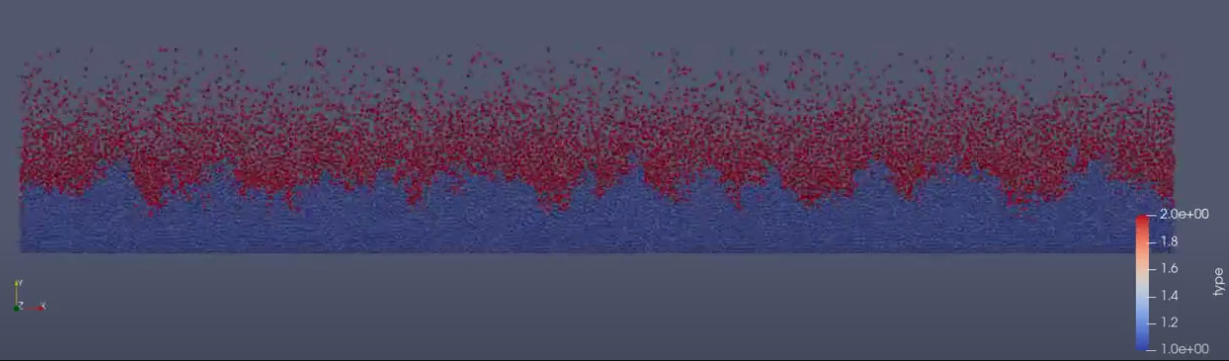
\includegraphics[width=0.9\textwidth]{../../res/rayleigh_bounce}
    \end{figure}
\end{frame}